\documentclass[11pt]{article}
\pagestyle{plain}
\usepackage{latexsym,exscale,amsfonts,amsmath,amssymb,array}
\usepackage{color}
\usepackage[colorlinks]{hyperref}
\setlength{\topmargin}{-2.3cm}
\setlength{\textheight}{23.8cm}
\setlength{\oddsidemargin}{-0.5cm}
\setlength{\textwidth}{17cm}
\setlength{\parindent}{0cm}
\setlength{\parskip}{.4cm}
\newcommand{\totaldiffx}{\frac{d}{dx}}
\newcommand{\pardiffx}{\frac{\partial}{\partial x}}
\newcommand{\luft}{\:\!}

\usepackage{graphicx}
\usepackage[latin1]{inputenc}
\usepackage{mathpazo}
\usepackage[T1]{fontenc}
\usepackage[comma,numbers,sort&compress]{natbib}


\begin{document}
\begin{center}
\large \bf Computational Astrophysics \rm \\
2019\\
{\small Exercises 08. Curve Fitting}
\end{center}

\begin{enumerate}

\item {\bf Curve Fitting: The $M_\mathrm{BH}-\sigma_*$ Relation }

In 2006, Greene and Ho \cite{Greene} studied the characteristics of 88 galaxies to show that there is an apparent relationship between the stellar velocity dispersion $\sigma_*$ in a galaxy bulge and the mass $M_\mathrm{BH}$ of the supermassive black hole at its
center, as shown in Figure \ref{fig:msigma} . This  is known as 
the $M_\mathrm{BH}-\sigma_*$ relation and is not yet  completely understood. 

The dataset used by Greene and Ho is available
online in various formats at
\url{http://vizier.cfa.harvard.edu/viz-bin/VizieR?-source=J/ApJ/641/L21}.


\vspace*{-0.3cm}
\begin{figure}[h!]
\centering
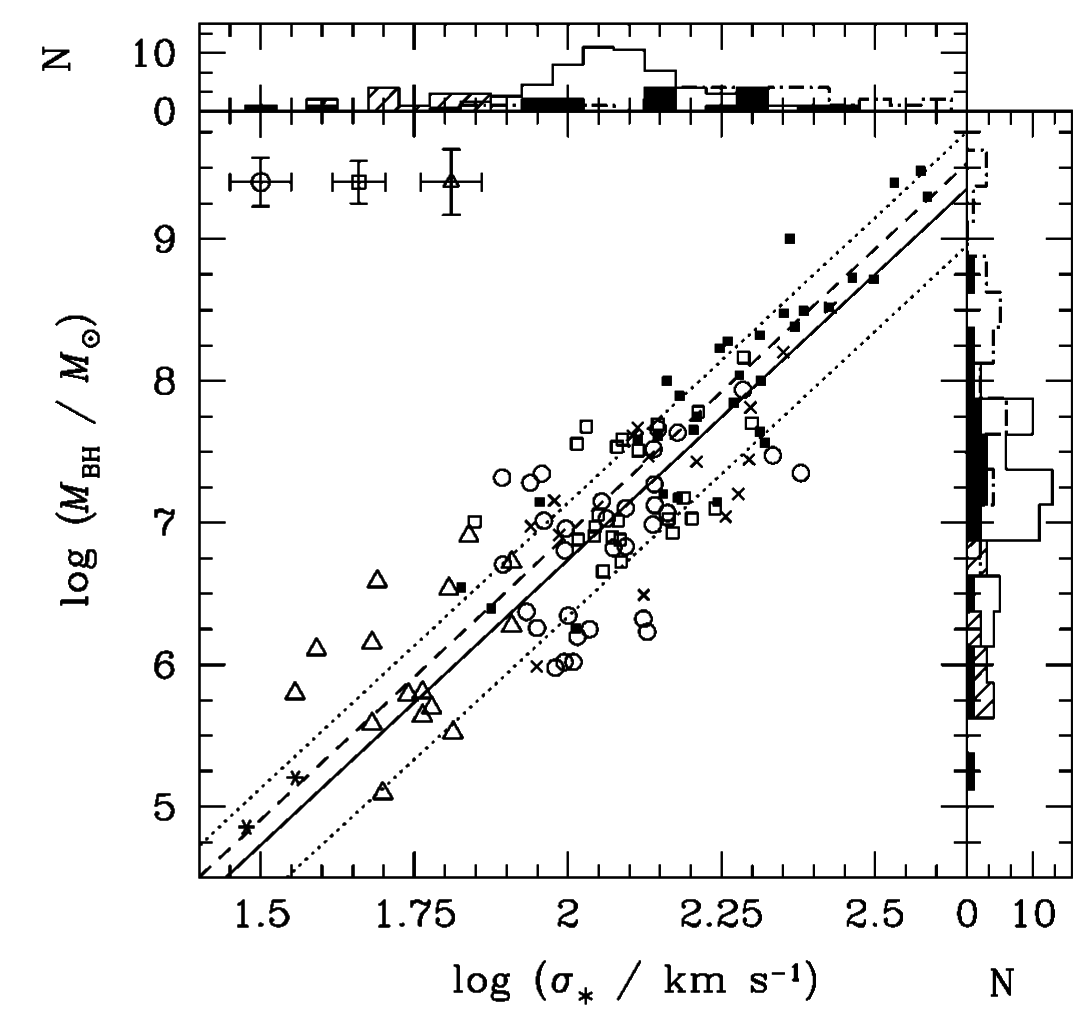
\includegraphics[width=0.55\textwidth]{msigma.png}
\caption{Figure taken from Greene \& Ho, ApJ 641:L21 (2006).}
\label{fig:msigma}
\end{figure}


\begin{enumerate}
\item[(a)] Go to \\
\url{http://cdsarc.u-strasbg.fr/viz-bin/cat/J/ApJ/641/L21}\\
In the tab "FTP" you can download the data files of the paper by Greene and Ho:\\
- ReadMe\\
- table1.dat\\

The ReadMe file describes the data stored in the table1.dat file. \\

In order to read the .dat file it can be used the {\tt AstroPy} package
or it is also possible to write a code to read it and store it in {\tt NumPy} arrays. \\

In the code directory of this lecture you can find a sample file ({\tt astropy\_reading.py}) using {\tt AstroPy} to read the data.

Make a plot of point ( no lines !) showing
$\log_\mathrm{10} M_\mathrm{BH}$ as a function of $\log_\mathrm{10}
\sigma_*$.

\item[(b)] Compute a linear regression fit 
to the data  (ignoring errors). Make a plot of data and fit. Compare your fit results to
that of Greene \& Ho (2006) in Figure \ref{fig:msigma}. (Maybe you will need some rescaling 
for a direct comparison.)

\item[(c)] Include the errors in $\log_\mathrm{10} \sigma_*$
  and $\log_\mathrm{10} M_\mathrm{BH}$ in your fit. There may be
  multiple errors given, use your judgement which ones to pick. How
  does this change your fit?
\end{enumerate}
\end{enumerate}
Happy Coding :) !
\begin{thebibliography} {9}
\bibitem{Greene} Greene, J. E. and Ho, L. C. \textit{The $M_{BH} - \sigma_*$ Relation in Local Active Galaxies}. ApJ 641 L21 (2006) \url{https://ui.adsabs.harvard.edu/abs/2006ApJ...641L..21G/abstract}
\end{thebibliography}
\end{document}
